
In this chapter we will show that the problem of computing the hybridization number of two rooted binary phylogenetic trees on the same set of taxa (\mh) has a constant factor polynomial-time approximation if and only if the problem of computing a minimum-size feedback vertex set in a directed graph (\dfvs) has a constant factor polynomial-time approximation. 


%A clue lies in the nature of the abstraction that is almost without exceptions used to compute hybridization number, \maaf. %, introduced in \cite{baroni05} (see Figure~\ref{fig:intro}). 
As we saw in the introduction chapter, computing the hybridization number of two trees $T_1$ and $T_2$ is essentially identical to the problem of cutting $T_1$ and $T_2$ into as few vertex-disjoint subtrees as possible such that the subtrees of $T_1$ are isomorphic to the subtrees of $T_2$ and - critically - a specific ``reachability'' relation on these subtrees is acyclic. The latter condition seems to be the core of the issue, because without this condition the problem would be no different to the problem of computing the rSPR distance, which as previously mentioned seems to be comparatively tractable. %(Note that the hybridization number of two trees can in general be much larger than their rSPR distance). 
The various FPT algorithms for computing hybridization number deal with the unwanted cycles in the reachability relation in a variety of ways but all resort to some kind of brute force analysis to optimally avoid (e.g. \cite{firststeps}) or break (e.g. \cite{hybridnet,whiddenFixed}) them.

In this chapter we demonstrate why it is so difficult to deal with the cycles. Problem \dfvs belongs to Karp's famous 1972 list of 21 NP-complete problems \cite{karp1972} and is also known to be APX-hard \cite{Kann}. However, despite almost forty years of attention it is still unknown whether \dfvs permits a constant approximation ratio i.e. whether it is in APX. %(The undirected variant of FVS, in contrast, appears to be significantly more tractable. It is 2-approximable even in the weighted case \cite{Bafna1999}).

By coupling the approximability of \mh to \dfvs we show that \mh is just as hard as a problem that has so far eluded the entire combinatorial optimization community. Specifically, we show that for every constant $c > 1$ and every $\epsilon > 0$ the existence of a polynomial-time $c$-approximation for \mh would imply a polynomial-time $(c + \epsilon)$-approximation for \dfvs. In the other direction we show that, for every $c > 1$, the existence of a polynomial-time $c$-approximation for \dfvs would imply a polynomial-time $6c$-approximation for \mh. In other words: \dfvs is in APX if and only if \mh is in APX. Hence a constant factor approximation algorithm for either problem would be a major breakthrough in theoretical computer science.


The structure of this chapter is as follows. We start with some definitions and describe two types of reductions that were used to show that \mh is fixed parameter tractable. We will need these in Section~\ref{sec:kernel}, where we show an improved bound on the sizes of reduced instances of \mh. Subsequently, we use these results to show an approximation-preserving reduction from \mh to \dfvs in Section~\ref{sec:2dfvs} and an approximation-preserving reduction from \dfvs to \mh in Section~\ref{sec:2minhybrid}. We conclude with a summary and some open problems.




%\section{Preliminaries}

After establishing the NP-hardness of \mh, the same authors showed that this problem is also fixed parameter tractable~\cite{bordewich07b}. They show how to reduce a pair of rooted binary phylogenetic $X$-trees~$T_1$ and~$T_2$, such that the number of leaves of the reduced trees is bounded by $14h(T_1,T_2)$, where $h(T_1,T_2)$ is the hybridization number of $T_1$ and~$T_2$. Since a brute-force algorithm can be used to solve the reduced instance, this leads to a fixed parameter tractable algorithm.

Let $A=(a_1,a_2,\ldots,a_n)$ be an $n$-chain that is common to two rooted binary phylogenetic $X$-trees $T_1$ and $T_2$ {with $n\geq 2$}, and let $\cF$ be an acyclic agreement forest for $T_1$ and $T_2$. We say that $A$ {\it survives} in $\cF$ if there exists an element in $\cF$ that is a superset of $\{a_1,a_2,\ldots,a_n\}$, while we say that $A$ is {\it atomized} in $\cF$ if each element in $\{a_1,a_2,\ldots,a_n\}$ is a singleton in $\cF$ (see Figure~\ref{fig:chains}). {Similarly, for a common pendant subtree $T$ of $T_1$ and $T_2$, we say that~$T$ survives in~$\cF$ if there is an element of~$\cF$ that is a superset of the label set of~$T$.}

\begin{figure}
    \centering
     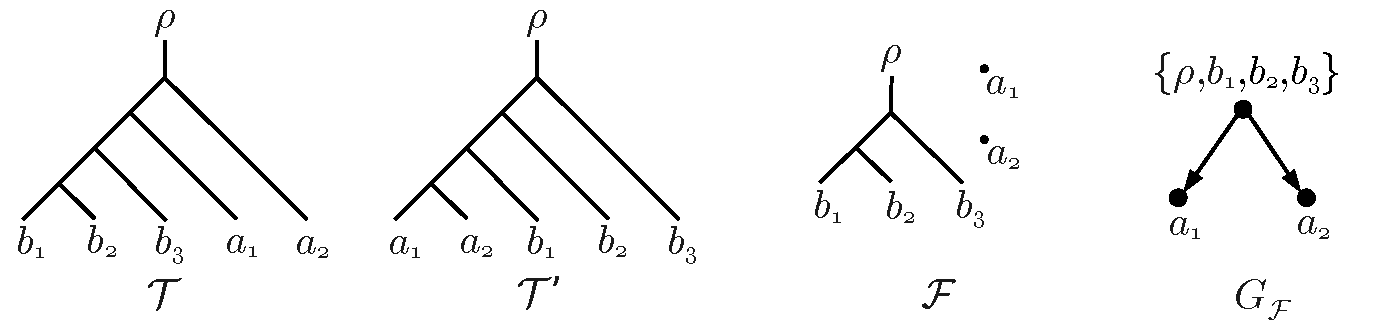
\includegraphics[scale=.5]{../figs/fig_chains}
    \caption{Two input trees~$T_1$ and $T_2$, an agreement forest~$\mathcal{F}$ for~$T_1$ and $T_2$ and the inheritance graph~$G_\mathcal{F}$. The trees have two common chains: $(a_1,a_2)$ and $(b_1,b_2,b_3)$. In the agreement forest~$\mathcal{F}$, chain $(a_1,a_2)$ is atomized while chain $(b_1,b_2,b_3)$ survives. The agreement forest~$\mathcal{F}$ is acyclic because~$G_\mathcal{F}$ is acyclic.}
    \label{fig:chains}
\end{figure}

The following lemma basically shows that we can reduce subtrees and chains. It differs slightly from the corresponding lemma in~\cite{bordewich07b} because we consider approximations while Bordewich and Semple considered only optimal solutions in that paper.

\begin{lemma}\label{lem:survives}\cite[Lemma 3.1]{bordewich07b}
Let~$\cF$ be an acyclic agreement forest for two trees~$T_1$ and~$T_2$. Then there exists an acyclic agreement forest~$\cF'$ for~$T_1$ and~$T_2$ with~$|\cF'|\leq |\cF|$ such that
\begin{itemize}
\item[1.] every common pendant subtree of~$T_1$ and~$T_2$ survives in~$\cF'$ and
\item[2.] every common $n$-chain of~$T_1$ and~$T_2$, with~$n\geq 3$, either survives or is atomized in~$\cF'$.
\end{itemize}
Moreover, $\cF'$ can be obtained from~$\cF$ in polynomial time.
\end{lemma}
\begin{proof}
Follows from the proof of~\cite[Lemma 3.1]{bordewich07b}. There are two differences with~\cite[Lemma 3.1]{bordewich07b}. Firstly, our result is slightly simpler because we consider two unweighted trees~$T_1$ and~$T_2$, while the authors of~\cite{bordewich07b} allow the unreduced trees~$T_1$ and $T_2$ to already have weights on 2-chains. Secondly,~\cite[Lemma 3.1]{bordewich07b} only shows the result for optimal agreement forests. However, a careful analysis of the proof of~\cite[Lemma 3.1]{bordewich07b} shows that it can also be used to prove this lemma.
\end{proof}

We are now ready to formally describe the aforementioned tree reductions. Let $T_1$ and $T_2$ be two rooted binary phylogenetic $X$-trees, $P$ a set that is initially empty and $w:P\rightarrow\mathbb{Z}^+$ a weight function on the elements in $P$.

\noindent{\bf Subtree Reduction.} Replace any maximal pendant subtree with at least two leaves that is common to $T_1$ and $T_2$ by a single leaf with a new label.

\noindent{\bf Chain Reduction.} Replace any maximal $n$-chain $(a_1,a_2,\ldots,a_n)$, with~$n\geq 3$, that is common to $T_1$ and $T_2$ by a $2$-chain with new labels $a$ and $b$. Moreover, add a new element $(a,b)$ with weight $w(a,b)=n-2$ to $P$.

Let $S_1$ and $S_2$ be two rooted binary phylogenetic $X'$-trees that have been obtained from $T_1$ and $T_2$ by first applying subtree reductions as often as possible and then applying chain reductions as often as possible. We call $S_1$ and $S_2$ the {\it reduced tree pair} with respect to  $T_1$ and $T_2$. Note that a reduced tree pair always has an associated set $P$ that contains one element for each chain reduction applied. Note that $S_1$ and $S_2$ are unambiguously defined (up to the choice of the new labels) because maximal common pendant subtrees do not overlap and maximal common chains do not overlap. Moreover, applications of the chain reduction can not create any new common pendant subtrees with at least two leaves. Hence, it is not necessary to apply subtree reductions again after the chain reductions.

Recall that every common $n$-chain, with~$n\geq 3$, either survives or is atomized (Lemma~\ref{lem:survives}). In~$S_1$ and~$S_2$, such chains have been replaced by weighted 2-chains. Therefore, we are only interested in acyclic agreement forests for~$S_1$ and~$S_2$ in which these weighted 2-chains either survive or are atomized. We therefore introduce a third notion of an agreement forest. Recall that~$P$ is the set of reduced (i.e. weighted) 2-chains. We say that an agreement forest~$\cF$ for~$S_1$ and~$S_2$ is {\it legitimate} if it is acyclic and every chain~$(a,b)\in P$ either survives or is atomized in~$\cF$.

\noindent Let $\cF$ be an agreement forest for $S_1$ and $S_2$. The {\it weight} of $\cF$, denoted by $w(\cF)$, is defined to be
\[w(\cF)=|\cF|-1+\sum_{(a,b)\in P: \mbox{ }(a,b)\textnormal{ is atomized in }\cF} w(a,b). \]
Lastly, we define $f(S_1,S_2)$ to be the minimum weight of a legitimate agreement forest for $S_1$ and $S_2$.

Then, the following lemma says that computing the hybridization number of~$T_1$ and~$T_2$ is equivalent to computing the minimum weight of a legitimate agreement forest for $S_1$ and $S_2$. The second part of the lemma is necessary to show that an approximation to a reduced instance $S_1$ and $S_2$ can be used to obtain an approximation to the original instance $T_1$ and $T_2$.

\begin{lemma}\label{l:preserving}\cite[Proposition 3.2]{bordewich07b}
Let $T_1$ and $T_2$ be a pair of rooted binary phylogenetic $X$-trees and let $S_1$ and $S_2$ be the reduced tree pair with respect to $T_1$ and $T_2$. Then
\begin{enumerate}
\item[(i)] $h(S_1,S_2) \leq f(S_1,S_2) = h(T_1,T_2)$ and
\item[(ii)] given a legitimate agreement forest~$\cF_S$ for~$S_1$ and~$S_2$, we can find, in polynomial time, an acyclic agreement forest~$\cF$ for $T_1$ and $T_2$ such that $|\cF| - 1 = w(\cF_S)$.
\end{enumerate}
\end{lemma}
% \begin{proof}
% In part (i), the inequality follows directly from the definition of~$f$ while the equality is equivalent to \cite[Proposition 3.2]{bordewich07b} if the unreduced trees~$T_1$ and $T_2$ are unweighted (i.e. if~$P$ is initially empty). Part (ii) follows from the proof of \cite[Proposition 3.2]{bordewich07b}.
% \end{proof}

The fixed parameter tractability of \mh now follows from the next lemma, which bounds the number of leaves in a reduced tree pair.

\begin{lemma}\cite[Lemma 3.3]{bordewich07b}\label{l:oldFPTfactor}
Let $T_1$ and $T_2$ be two rooted binary phylogenetic $X$-trees, $S_1$ and $S_2$ the reduced tree pair with respect to $T_1$ and $T_2$, and~$X'$ the label set of~$S_1$ and~$S_2$. If $h(T_1,T_2)>0$, then $|X'|<14h(T_1,T_2)$.
\end{lemma}

\noindent We show in Section~\ref{sec:kernel} that the reduced trees have at most $9h(T_1,T_2)$ leaves. This improved bound will be important in the approximation-preserving reductions we give later in the chapter.






\section{An improved bound on the size of reduced instances of \mh}\label{sec:kernel}

We start with some definitions and an intermediate result. The bound on the size of the reduced instance will be proven in Theorem \ref{thm:newKernel}.

An $r$-\emph{reticulation generator} (for short, {\it $r$-generator}) is defined to be a directed acyclic multigraph with  a single vertex of indegree~0 and  outdegree~1 {(which we can think of as being labelled by $\rho$)}, precisely~$r$ reticulation vertices (indegree~2 and outdegree at most~1), and apart from that only vertices of indegree~1 and outdegree~2 \cite{KelkScornavacca2011}.  The \emph{sides} of an $r$-generator are its edges (the \emph{edge} sides) and its vertices of indegree-2 and outdegree-0 (the \emph{node sides}). Adding a set of labels $L$ to an edge side $(u, v)$ of an $r$-generator involves subdividing $(u, v)$ to a path of $|L|$ internal vertices and, for each such internal vertex $w$, adding a new leaf $w'$, an edge $(w, w')$, and labeling $w'$ with some taxon from $L$ (such that~$L$ bijectively labels the new leaves). On the other hand, adding a label $l$ to a node side $v$ consists of adding a new leaf $y$, an edge $(v, y)$ and labeling $y$ with $l$.

\begin{lemma}\label{lem:generator}
Let $T_1$ and $T_2$ be two rooted binary phylogenetic $X$-trees with no common pendant subtrees with at least~2 leaves and let~$H$ be a hybridization network that displays~$T_1$ and~$T_2$ with a minimum number of hybridization vertices. Then the network~$H'$ obtained from~$H$ by deleting all {$|X|$} leaves and suppressing each resulting vertex~$v$ with $d^+(v)=d^-(v)=1$ is an $h(H)$-generator.
\end{lemma}
\begin{proof}
By construction, $H'$ contains the same number of hybridization vertices as~$H$. Additionally,
by the definition of a binary hybridization network, no vertex has indegree~2 and outdegree greater than~1, indegree greater than~2, or indegree and outdegree both~1. Now, we claim that~$H'$ does not have any vertex with indegree~1 and outdegree~0. To see that this holds, suppose that there exists a vertex~$v$ in~$H'$ such that $d^-(v)= 1$ and $d^+(v)= 0$. Then~$v$ has two children in~$H$. Since $d^+(v)= 0$ in~$H'$, no hybridization vertex can be reached by a directed path from~$v$ in~$H$. This means that the subnetwork of~$H$ rooted at~$v$ is actually a rooted tree, contradicting the fact that~$T_1$ and~$T_2$ do not have any common pendant subtree with two or more leaves. We may thus conclude that~$H'$ conforms to the definition of an $h(H)$-generator.
\end{proof}

Conversely, by inverting the operations of suppression and deletion,~$H$ can be obtained from the $h(H)$-generator~$H'$ associated with~$H$ by adding leaves to its sides (in the sense described at the start of this section).
{This relies on the intuitive fact that modulo leaves and suppression the $h(H)$-generator obtained in Lemma \ref{lem:generator} has essentially the same topology as $H$. A similar technique was described in~\cite{KelkScornavacca2011} in a somewhat different context.}\\

\begin{theorem}\label{thm:newKernel}
Let $T_1$ and $T_2$ be two rooted binary phylogenetic $X$-trees and~$S_1$ and~$S_2$ the reduced tree pair on~$X'$ with respect to~$T_1$ and~$T_2$. If $h(T_1,T_2)>0$, then $|X'|< 9h(T_1,T_2)$.
\end{theorem}
\begin{proof}
Let $H'$ be the $h(H)$-generator that is associated with a hybridization network $H$ for $S_1$ and $S_2$ whose number of hybridization vertices is minimized, i.e., $h(H)=h(S_1,S_2)$. By definition, $H'$ has the following vertices:
\begin{itemize}
\item $r=h(H)$ reticulations; in particular $r_0$ reticulations with indegree 2 and outdegree 0 and $r_1$ reticulations with indegree 2 and outdegree 1,
\item $s$ vertices with indegree 1 and outdegree 2, and
\item one {vertex labelled $\rho$} with indegree 0 and outdegree 1.
\end{itemize}
The total indegree of~$H'$ is $2r_0 + 2r_1 + s$. The total outdegree of~$H'$ is $ r_1 + 2s + 1$. Hence, $2r_0 + 2r_1 + s = r_1 + 2s + 1$ implying $s = 2r_0 + r_1 - 1$. Moreover, the total number of edges of~$H'$, $|E(H')|$, equals the total indegree and, therefore,
\begin{equation}\label{eq:edges}
|E(H')|=2r_0 + 2r_1 + s=2r_0 + 2r_1 +2r_0 + r_1 - 1=4r_0+3r_1-1.\\
\end{equation}

Note that for each of the $r_0$ node sides~$v$ in $H'$ the child of $v$ in $H$ is a single leaf. Moreover, each edge side in $H'$ cannot correspond to a directed path in $H$ that consists of more than three edges since, otherwise, $S_1$ and $S_2$ would have a common $n$-chain, with $n\geq 3$. Thus,~$H$ can have at most two leaves per edge side of~$H'$ and one leaf per node side of~$H'$. Thus, the total number of leaves~$|X'|$ of~$H$ is bounded by

\begin{align*}
|X'|&\leq 2|E(H')| + r_0 \\
&= 2(4r_0 + 3r_1 - 1) + r_0\\
&= 9r_0 + 6r_1 - 2\\
& \leq 9r - 2\\
&< 9h(S_1,S_2)\\
&\leq 9h(T_1,T_2),
\end{align*}
where the last inequality follows from Lemma~\ref{l:preserving}.
\end{proof}






\section{An approximation-preserving reduction from \mh to \dfvs}\label{sec:2dfvs}

We start by proving the following theorem, which refers to {\sc wDFVS}, the \emph{weighted} variant of {\sc DFVS} where every vertex is attributed a weight and the weight of a feedback vertex set is simply the sum of the weights of its constituent vertices. Later in the section we will prove a corresponding result for {\sc DFVS}.

\begin{theorem}\label{t:Hybrid2DFVS} If, for some~$c\geq 1$, there exists a polynomial-time $c$-approximation for {\sc wDFVS}, then there exists a polynomial-time $6c$-approximation for \mh.
\end{theorem}

Throughout this section, let~$T_1$ and~$T_2$ be two rooted binary phylogenetic $X$-trees, and let $S_1$ and $S_2$ be the reduced tree pair on $X'$ with respect to $T_1$ and $T_2$. Using Lemma~\ref{lem:survives}, we assume throughout this section without loss of generality that~$T_1$ and~$T_2$ do not contain any common pendant subtrees with at least two leaves. Thus, the reduced tree pair $S_1$ and $S_2$ can be obtained from $T_1$ and $T_2$ by applying the chain reduction only.

Before starting the proof, we need some additional definitions and lemmas. We say that a common chain $(a,b)$ of $S_1$ and $S_2$ is a {\it reduced chain} if it is not a common chain of $T_1$ an $T_2$. Otherwise, $(a,b)$ is an {\it unreduced chain}, see figure \ref{fig:chains}. Furthermore, a taxon $\ell\in X'\cup\{\rho\}$, is a {\it non-chain taxon} if it does not label a leaf of a reduced or unreduced chain of $S_1$ and $S_2$. Now, let $\cB_S$ be the forest that exactly contains the following elements:
\begin{enumerate}
\item for each non-chain taxon $\ell$ of $S_1$ and $S_2$, a {\it non-chain element} $\{\ell\}$, and
\item for each reduced and unreduced chain $(a,b)$ of $S_1$ and $S_2$, an element $\{a,b\}$.
\end{enumerate}
Clearly, $\cB_S$ is an agreement forest for $S_1$ and $S_2$, and we refer to it as a {\it chain forest} for $S_1$ and $S_2$.
Now, obtain $\cB_T$ from $\cB_S$ by replacing  each element in $\cB_S$ that contains two labels of a reduced chain, say $(a,b)$, of $S_1$ and $S_2$ with the label set that precisely contains all labels of the common $n$-chain that has been reduced to $(a,b)$ in the course of obtaining $S_1$ and $S_2$ from $T_1$ and $T_2$, respectively. The set $\cB_T$ is an agreement forest for $T_1$ and $T_2$, and we refer to it as a {\it chain forest} for  $T_1$ and $T_2$. Since the chain reduction can be performed in polynomial time~\cite{bordewich07b}, the chain forests $\cB_S$ and $\cB_T$ can also be calculated in polynomial time from $T_1$ and $T_2$. Lastly, each element in $\cB_T$ whose members label the leaves of a common $n$-chain in $T_1$ and $T_2$ with $n\geq 2$  is referred to as a {\it chain element}.

The next lemma bounds the number of elements in a chain forest.

\begin{lemma}\label{l:B_bound}
Let $T_1$ and $T_2$ be two rooted binary phylogenetic $X$-trees. Let $S_1$ and $S_2$ be the reduced tree pair with respect to $T_1$ and $T_2$. Furthermore, let $\cB_S$ and $\cB_T$ be the chain forests for $S_1$ and $S_2$, and $T_1$ and $T_2$, respectively. Then $|\cB_T| =|\cB_S|< 5h(T_1,T_2)$.
\end{lemma}

\begin{proof}
By construction of $\cB_T$ from $\cB_S$, it immediately follows that $|\cB_T| =|\cB_S|$. To show that $|\cB_S|< 5h(T_1,T_2)$ let $H$ be a hybridization network that displays $S_1$ and $S_2$ such that its number of hybridization vertices is minimized over all such networks. Furthermore, let $H'$ be the $h(H)$-generator associated with $H$.
As in the proof of Theorem \ref{thm:newKernel}, let $r_0$ be the number of node sides, i.e. reticulations with indegree~2 and outdegree~0, in $H'$ and let $r_1$ be the number of reticulations in $H'$ with indegree~2 and outdegree~1. Again, $r_0 + r_1 = h(H')= h(S_1,S_2)$. Recall that, to obtain~$H$ from~$H'$, we add one leaf to each node side of~$H'$, corresponding to a singleton in~$\cB_S$, and at most two leaves to each edge side of~$H'$. Each edge side of $H'$ to which we add two taxa corresponds to a 2-chain of $S_1$ and $S_2$ and, therefore, to a single element in $\cB_S$. Hence, using \eqref{eq:edges} and Lemma~\ref{l:preserving}, we have
\[|\cB_T|=|\cB_S|  \leq  |E(H')| +r_0 = 5r_0 + 3r_1 -1 < 5(r_0+r_1) = 5 h(S_1,S_2) \leq 5 h(T_1,T_2).\]
\end{proof}

Consider again the chain forest $\cB_T$ for $T_1$ and $T_2$. We define a {\it $\cB_T$-splitting} as an acyclic agreement forest for $T_1$ and $T_2$ that can be obtained from $\cB_T$ by repeated replacements of a chain element $\{a_1,a_2,\ldots,a_n\}$ with the elements $\{a_1\},\{a_2\},\ldots,\{a_n\}$.

\begin{lemma}\label{l:bTprops}
Let $\cB_T$ be the chain forest for two rooted binary phylogenetic $X$-trees $T_1$ and $T_2$. Let $\{a_1,a_2,\ldots,a_n\}$ be a chain  element in $\cB_T$, and let {$\cL_j$ be a non-chain element in $\cB_T$}. Furthermore, let $\cB_{T'}=(\cB_T-\{\{a_1,a_2,\ldots,a_n\}\})\cup\{\{a_1\},\{a_2\},\ldots,\{a_n\}\}$. Then, for the inheritance graph $G_{B_{T'}}$ we have
\begin{enumerate}
\item no directed cycle of $G_{\cB_{T'}}$ passes through an element of $\{\{a_1\},\{a_2\},\ldots,\{a_n\}\}$ and
\item no directed cycle of $G_{\cB_T}$ passes through {$\cL_j$}.
\end{enumerate}
\end{lemma}
\begin{proof}
{By the definition of $\cB_T$, note that $|\cL_j|=1$. If $\cL_j=\{\rho\}$, then the indegree of $\cL_j$ is 0 in $G_{\cB_T}$. Otherwise, if $\cL_j\ne\{\rho\}$, then its element labels a leaf of $T_1$ and $T_2$  and, thus the outdegree of $\cL_j$ is 0 in $G_{\cB_T}$.} Furthermore, since each element in $\{\{a_1\},\{a_2\},\ldots,\{a_n\}\}$ also labels a leaf of $T_1$ and $T_2$, the outdegree of the vertices $a_1,a_2,\ldots,a_n$ in $G_{\cB_{T'}}$ is 0. This establishes the lemma.
\end{proof}

Let $\opt$ denote the size of a $\cB_T$-splitting of smallest size.

\begin{lemma}\label{l:bSplitting}
Let $T_1$ and $T_2$ be two rooted binary phylogenetic $X$-trees, and let $\cB_T$ be the chain forest for $T_1$ and $T_2$. Then, $\opt<6h(T_1,T_2)$.
\end{lemma}
\begin{proof}
Let $\cF_{T_1}$ be a maximum acyclic agreement forest for $T_1$ and $T_2$. In this proof, we see an agreement forest as a collection of trees. Thus, $\cF_{T_1}$ can be obtained from $T_1$ (or equivalently from $T_2$) by deleting an $(|\cF_{T_1}|-1)$-sized subset, say $E_{\cF_{T_1}}$, of the edges of $T_1$ and cleaning up. Similarly, $\cB_T$ can be obtained from $T_1$ (or equivalently from $T_2$) by deleting a $(|\cB_T|-1)$-sized subset, say $E_{\cB_T}$, and cleaning up. Now consider the forest $\cB_{T'}$ obtained from $T_1$ by removing the edge set $E_{\cF_{T_1}} \cup E_{\cB_T}$ and cleaning up.

We claim that $\cB_{T'}$ is a $\cB_T$-splitting. To see this, first observe that $\cB_{T'}$ is an acyclic agreement forest for $T_1$ and $T_2$ because it can be obtained by removing edge set~$E_{\cB_T}$ from~$\cF_{T_1}$ and cleaning up. Hence, to show that $\cB_{T'}$ is a $\cB_T$-splitting, it is left to show that it can be obtained from $\cB_T$ by repeated replacements of a caterpillar on $\{a_1,a_2,\ldots,a_n\}$ by isolated vertices $\{a_1\},\{a_2\},\ldots,\{a_n\}$. By its definition, $\cB_{T'}$ can be obtained from $\cB_T$ by removing edges and cleaning up. Thus, what is left to prove is that each chain either survives or is atomized. For $n$-chains with~$n\geq 3$, this follows from Lemma~\ref{lem:survives}, and for $n=2$ it is clear because $\cB_{T'}$ can be obtained by removing edges from $\cB_T$ in which each 2-chain is a component on its own.

As the size of $\cB_{T'}$ is equal to the number of edges removed to obtain it from $T_1$ plus one, we have:
\[|\cB_{T'}| \leq |E_{\cF_{T_1}}| + |E_{\cB_T}| +1 = |\cF_{T_1}| - 1 + |\cB_T| < h(T_1,T_2) + 5 h(T_1,T_2) = 6 h(T_1,T_2),\]
{where Lemma \ref{l:B_bound} is used to bound $|\cB_T|$.} This establishes the lemma.
\end{proof}

We are now in a position to prove the main result of this section.
\begin{proof}[Proof of Theorem~\ref{t:Hybrid2DFVS}]
Throughout this proof, let $n\geq 2$. Furthermore, let $\cB_T$ be the chain forest for $T_1$ and $T_2$, and let $G$ be the graph obtained from the inheritance graph $G_{\cB_T}$ by subsequently
\begin{enumerate}
\item weighting each vertex that corresponds to a common $n$-chain $(a_1,a_2,\ldots,a_n)$ of $T_1$ and $T_2$  with weight $n$;
\item deleting each vertex that  corresponds to a non-chain taxon in $\cB_T$; and
\item for each remaining vertex $v$, creating a new vertex $\bar{v}$ with weight $1$ and two new edges $(v,\bar{v})$ and $(\bar{v},v)$.
\end{enumerate}
Furthermore, let $w$ be the weight function on the vertices of $G$. See Figure~\ref{fig:todfvs1} for an example of the construction of~$G$. We call the added vertices $\bar{v}$ the \emph{barred} vertices of $G$. Note that each common $n$-chain of $T_1$ and $T_2$ is represented by a vertex and its barred vertex in $G$. As $\cB_T$ can be calculated in polynomial time, the construction of $G$ also takes polynomial time, {and the size of $G$ is clearly polynomial in the cardinality of $\cB_T$}.

\begin{figure}
    \centering
     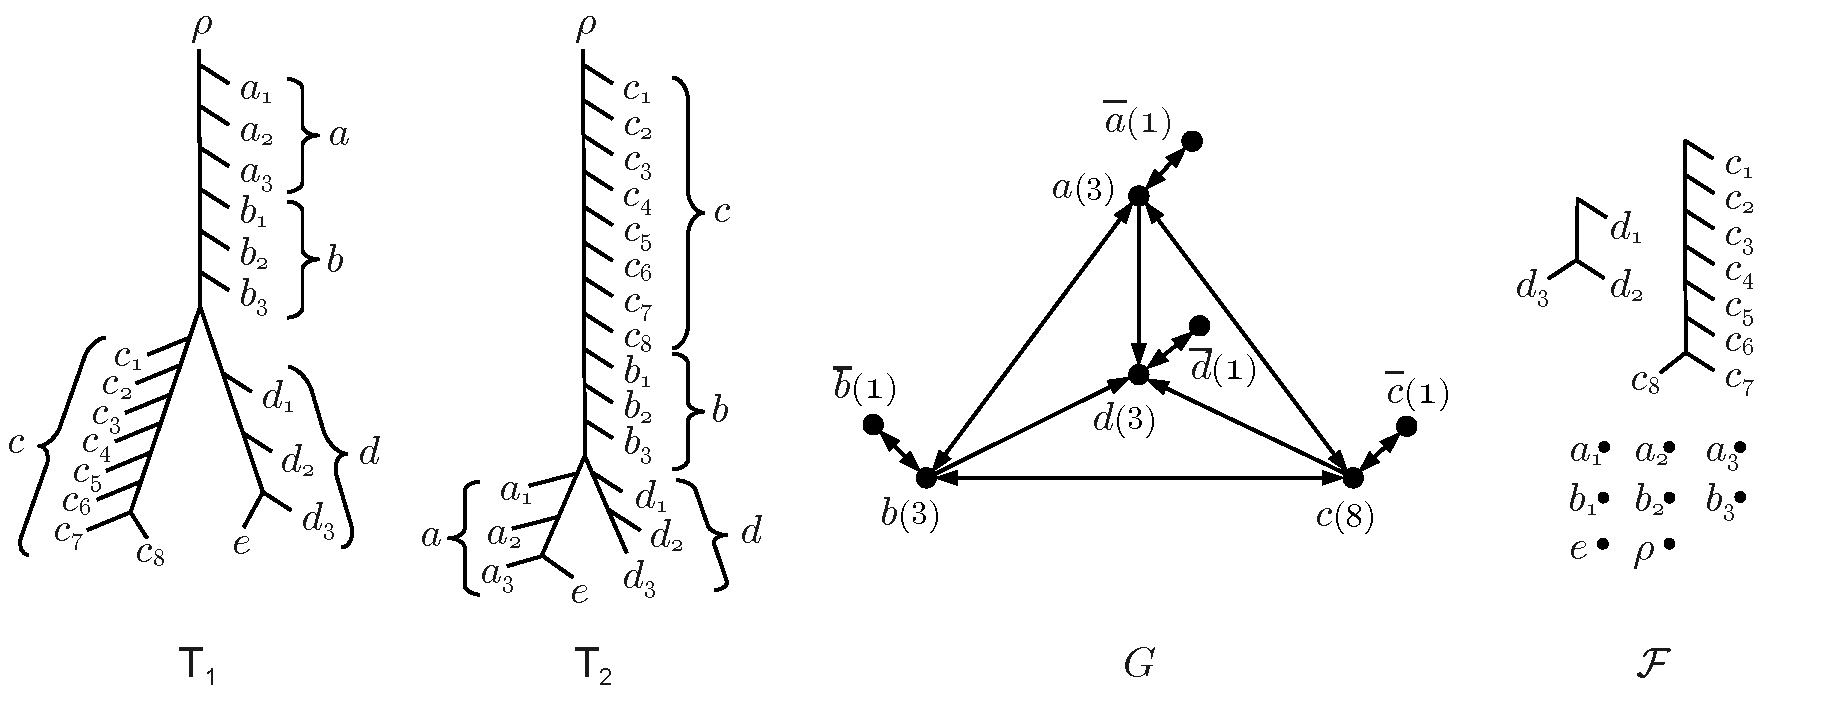
\includegraphics[scale=.4]{../figs/fig_todfvs1v5}
    \caption{Two input trees~$T_1$ and $T_2$, their graph~$G$ (with weights between parentheses) and an acyclic agreement forest~$\mathcal{F}$ of~$T_1$ and $T_2$. Note that~$\cF$ is a ${\cB_T\text{-splitting}}$ because it can be obtained from the chain forest $\cB_T$  by atomizing chains $a=(a_1,\ldots,a_3)$ and $b=(b_1,\ldots,b_3)$. Also note that~$\cF$ has~10 components, which is equal to the weight of a minimum feedback vertex set $\{a,b,\bar{c},\bar{d}\}$ of $G$, 8, plus 2, for two non-chain taxa ($\rho$ and~$e$).
}
 \label{fig:todfvs1}
\end{figure}

Now, regarding $G$ as an instance of {\sc wDFVS}, we claim the following.

\noindent{\bf Claim.} There exists a $\cB_T$-splitting of size $k+s$, where $s$ is the number of non-chain elements in $\cB_T$, if and only if $G$ has a FVS of weight $k$.

{Suppose that $\cB_{T'}$ is a $\cB_T$-splitting of size~$k+s$. Hence, $k$ is equal to the number of chain elements in $\cB_T$ that are also elements in $\cB_{T'}$ plus the total number of leaves in common $n$-chains that are atomized in $\cB_{T'}$. Let ${T_2}$ be the forest that has been obtained from $\cB_{T'}$ by deleting all singletons, and let $G_{\bar{\cB}_{T_2}}$ be its inheritance graph. Since $G_{\cB_{T'}}$ is acyclic, $G_{\bar{\cB}_{T_2}}$ is also acyclic. Now, let $G'$ be the directed graph that has been obtained from $G$ in the following way. For each non-barred vertex $v$ in $G$, delete $v$ if $v$ corresponds to an $n$-chain of $T_1$ and $T_2$ that is atomized in $\cB_{T'}$, and delete $\bar{v}$ if $v$ corresponds to an $n$-chain of $T_1$ and $T_2$ that is not atomized in $\cB_{T'}$}. Note that for each 2-cycle $(v,\bar{v},v)$ of $G$ either $v$ or $\bar{v}$ is not a vertex of $G'$ because each $n$-chain that is common to $T_1$ and $T_2$ is either atomized or not in $\cB_{T'}$. {This 
in turn implies that $G'$ is acyclic because  $G_{\bar{\cB}_{T_2}}$ is isomorphic to $G'\backslash \bar{V}$, where $\bar{V}$ precisely contains all barred vertices of $G'$. Hence, an FVS of $G$, say $V$, contains each vertex of $G$ that is not a vertex of $G'$. Furthermore, by the weighting of $G$, it follows that the weight of $V$ is exactly $k$.}

Conversely, suppose that there exists an FVS of $G$, say $V$, with weight $k$. This implies that we can remove a set $V_1$ of barred vertices  and a set  $V_2=V\backslash V_1$ of non-barred vertices such that $\sum_{v_i\in V_2}w(v_i)+|V_1|=k$ and the graph  $G'=G\backslash V$ is acyclic. For each vertex $v_i\in V_2$, let $A_i=(a_{i,1},a_{i,2},\ldots,a_{i,n_i})$ be its associated common chain of $T_1$ and $T_2$, and let $w(v_i)$ be the number of elements in $A_i$. Furthermore, let $V_1'$ be the subset of $V_1$ that contains precisely each vertex $\bar{v}$ of $V_1$ for which $v\notin V_2$. If $|V_1'|<|V_1|$, then it is easily checked that $V_1'\cup V_2$ is an FVS of $G$ whose weight is strictly less than $k$. Therefore, we may assume for the remainder of this proof that $|V_1'|=|V_1|$. Now, let $\cB_{T'}$ be the forest that has been obtained from $\cB_T$ in the following way. For each vertex $v_i$ in $V_2$, replace $A_i$ in $\cB_T$ with the elements $\{a_{i,1}\},\{a_{i,2}\},\ldots,\{a_{i,n_i}\}$. Thus, 
$A_i$ is atomized in  $\cB_{T'}$. We next construct the inheritance graph $G_{\cB_{T'}}$ from $G_{\cB_T}$. For each vertex $v$ of $G_{\cB_T}$ that corresponds to a common $n$-chain $(a_1,a_2,\ldots,a_n)$ of $T_1$ and $T_2$ that is atomized in $\cB_{T'}$, replace $v$ with the vertices $a_1,a_2,\ldots,a_n$, delete each edge $(v,w)$ of $G_{\cB_T}$, and replace each edge $(u,v)$ of $G_{\cB_T}$ with the edges $(u,a_1),(u,a_2),\ldots,(u,a_n)$. By the proof of Lemma~\ref{l:bTprops}, the vertices $a_1,a_2,\ldots,a_n$ have outdegree 0 in $G_{\cB_T'}$. Noting that there is a natural bijection between the cycles in $G_{\cB_T}$ and the cycles in $G$ that do not pass through any barred vertex, it follows that, as $G'$ is acyclic, $G_{\cB_T'}$ is also acyclic. Hence, $\cB_{T'}$ is a $\cB_T$-splitting for $T_1$ and $T_2$. The claim now follows from
$$|\cB_{T'}|=s+\sum_{v_i\in V_2}w(v_i)+|V_1|=s+k.$$

It remains to show that the reduction is approximation preserving. Suppose that there exists a polynomial-time $c$-approximation for {\sc wDFVS}. Let $k$ be the weight of a solution returned by this algorithm, and let $k^*$ be the weight of an optimal solution. By the above claim, we can then construct a solution to {\sc MAAF} of size $k+s$, from which we can obtain a solution to \mh with value $k+s-1$ by Theorem~\ref{t:hybrid}. We have,
$$k + s - 1 < ck^*+s\leq ck^*+cs=c(k^*+s)=c\cdot\opt$$
and, thus, a constant factor $c$-approximation for finding an optimal $\cB_T$-splitting. Now, by Lemma~\ref{l:bSplitting},
$$k + s - 1\leq c\cdot\opt\leq 6c\cdot h(T_1,T_2),$$
thereby establishing that, if there exists a polynomial-time $c$-approximation for {\sc wDFVS}, then there exists a polynomial-time $6c$-approximation for \mh. This concludes the proof of the theorem.
\end{proof}

It is not too difficult to extend Theorem \ref{t:Hybrid2DFVS} to {\sc DFVS} i.e. the unweighted variant of directed feedback vertex set.

\begin{theorem}
\label{t:Hybrid2DFVSunweight} If, for some~$c\geq 1$, there exists a polynomial-time $c$-approximation for {\sc DFVS}, then there exists a polynomial-time $6c$-approximation for \mh.
\end{theorem}
\begin{proof}
In the proof of Theorem \ref{t:Hybrid2DFVS} we create an instance $G$ of {\sc wDFVS}. Let
$w$ be the weight function on the vertices of $G$. Note that the function is non-negative
and integral and for every vertex $v \in G$, $w(v) \leq |X|$ i.e. the weight function is polynomially bounded
in the input size. We create an instance $G'$ of DFVS as follows. For each vertex $v$ in $G$ we create $w(v)$ vertices in $G'$
$v_1, \ldots, v_{w(v)}$. For each edge $(u,v)$ in $G$ we introduce edges
$\{ (u_i, v_j) | 1 \leq i \leq w(u), 1 \leq j \leq w(v) \}$ in $G'$. Solutions to {\sc wDFVS($G$)}
and {\sc DFVS($G'$)} are very closely related, {which allows us to construct in polynomial-time a $c$-approximation
algorithm for {\sc wDFVS} from a $c$-approximation from {\sc DFVS}}.
Formally, what
we will demonstrate is an L-reduction \cite{papayanna} from {\sc wDFVS} to {\sc DFVS} 
%with coefficients $\alpha = \beta = 1$ 
which works for instances with polynomially-bounded weights. Specifically, consider any
feedback vertex set $F'$ of $G'$ of size $k$. We create a feedback vertex set $F$ of
$G$ as follows. For each vertex $v \in G$, we include $v$ in $F$ if and only if \emph{all}
the vertices $v_1, \ldots, v_{w(v)}$ are in $F'$. Note that the weight of $F$ is
less than or equal to $k$. To see that $F$ is a feedback vertex set, suppose
some cycle $C = u,v,w,\ldots,u$ survives in $G$. But then, for each vertex $u \in C$,
some vertex $u_i$ survives in $G'$, which means a cycle also survived in $G'$, contradicting
the assumption that $F'$ is a feedback vertex set. In the other direction, observe that any weight $k$ feedback vertex set $F$ of $G$ can be transformed into a feedback vertex set $F'$ of
$G'$ with size $k$ as follows: for each $v \in F$, place all $v_{1}, \ldots, v_{w(v)}$ in $F'$.
\end{proof}

Notice that Theorem~\ref{t:Hybrid2DFVS} does not hold only for constant~$c$, an observation used in the next corollary.

\begin{corollary}
\label{cor:approxalg}
There exists a polynomial-time $\text{O}( \log r \log \log r)$-approximation for \mh, where
$r = h(T_1, T_2)$
\end{corollary}
\begin{proof}
In \cite{dfvsApprox}, which extended \cite{dfvsSeymour}, a polynomial-time approximation algorithm for wDFVS is presented whose approximation ratio is $\text{O}( \min( \log |V| \log \log |V|, \log \tau^{*} \log \log \tau^{*}) )$, where $|V|$ is the number of vertices in the wDFVS instance and $\tau^{*}$ is the optimal \emph{fractional} solution value of the problem. We show that in the wDFVS instance $G$ that we create in the proof of Theorem~\ref{t:Hybrid2DFVS},
both the number of vertices in $G$ and the weight of the optimal fractional solution value of {\sc wDFVS}$(G)$ are $\text{O}(r)$. To see that $G$ has at most $\text{O}(r)$ vertices, observe that $G$ contains two vertices for every chain element in
the chain forest $\cB_T$, and that (by Lemma \ref{l:B_bound}) $|\cB_T| < 5r$.
Secondly, recall from Lemma \ref{l:bSplitting} that $\opt < 6r$. By construction, $\opt$ is
an upper bound on the optimum solution value of {\sc wDFVS}$(G)$, hence on $\tau^{*}$.
Thus, given $G$ as input, the algorithm in \cite{dfvsApprox} constructs
a feedback vertex set that is at most a factor $\text{O}( \log r \log \log r)$ larger than the true
optimal solution of {\sc wDFVS}$(G)$. As shown in the proof of Theorem
\ref{t:Hybrid2DFVS} this can be used to obtain an approximation ratio at most 6 times
larger for {\sc MAAF}, which is clearly also $\text{O}( \log r \log \log r)$.
\end{proof}

\noindent
Finally, note that for a given instance the actual approximation ratio obtained by Corollary \ref{cor:approxalg} will sometimes be determined by $|V|$, and sometimes by $\tau^{*}$,
and can potentially be significantly smaller than $\text{O}( \log r \log \log r)$. For example,
if there are very few chains in the chain forest, but they are all extremely long, then it can
happen that $|V| << \tau^{*}$. Conversely, if the chain forest contains many short chains, and
only a small number of them need to be atomized to attain acyclicity, then it can happen
that $\tau^{*} << |V|$.





\section{An approximation-preserving reduction from \dfvs to \mh}\label{sec:2minhybrid}

In this section we prove the following theorem.

\begin{theorem}
\label{theorem:dfvsToHybrid}
If, for some constant~$c\geq 1$, there exists a polynomial-time $c$-approximation algorithm for \mh, then there exists a polynomial-time $(c+\epsilon)$-approximation algorithm for {\sc DFVS} for all~$\epsilon>0$.
\end{theorem}
\begin{proof}
We show an approximation preserving reduction from {\sc DFVS} to {\sc MAAF}. The theorem then follows because of the equivalence of MAAF and \mh described in Theorem~\ref{t:hybrid}.

Let~$D=(V,A)$ be an instance of {\sc DFVS}. First we transform~$D$ into an auxiliary graph~$D'=(V',A')$. For a vertex~$v$ of~$D$, we denote the parents of~$v$ as $u_1,u_2,\ldots,u_{d^-(v)}$ and the children of~$v$ as $w_1,w_2,\ldots,w_{d^+(v)}$ (To facilitate the exposition, we assume a total order on the parents of each vertex and on the children of each vertex.). We construct the graph~$D'$ as follows. For every vertex~$v\in V$,~$D'$ has vertices $v_{\text{in}}^{u_1},v_{\text{in}}^{u_2},\ldots,v_{\text{in}}^{u_{d^-(v)}}$, vertices~$v^-$ and~$v^+$ as well as vertices $v_{\text{out}}^{w_1},v_{\text{out}}^{w_2},\ldots,v_{\text{out}}^{w_{d^+(v)}}$. The edges of~$D'$ are as follows. For each vertex~$v\in V$,~$D'$ has edges from each of $v_{\text{in}}^{u_1},v_{\text{in}}^{u_2},\ldots,v_{\text{in}}^{u_{d^-(v)}}$ to~$v^-$, an edge from~$v^-$ to~$v^+$ and edges from~$v^+$ to each of $v_{\text{out}}^{w_1},v_{\text{out}}^{w_2},\ldots,v_{\text{out}}^{w_{d^+(v)}}$. In addition, for each edge~$(u,v)$ of~$D$, there is an 
edge~$(u_\text{out}^{v},v_\text{in}^u)$ in~$D'$. This concludes the construction of~$D'$. An example is given in Figure~\ref{fig:reduction1}.

\begin{figure}
    \centering
    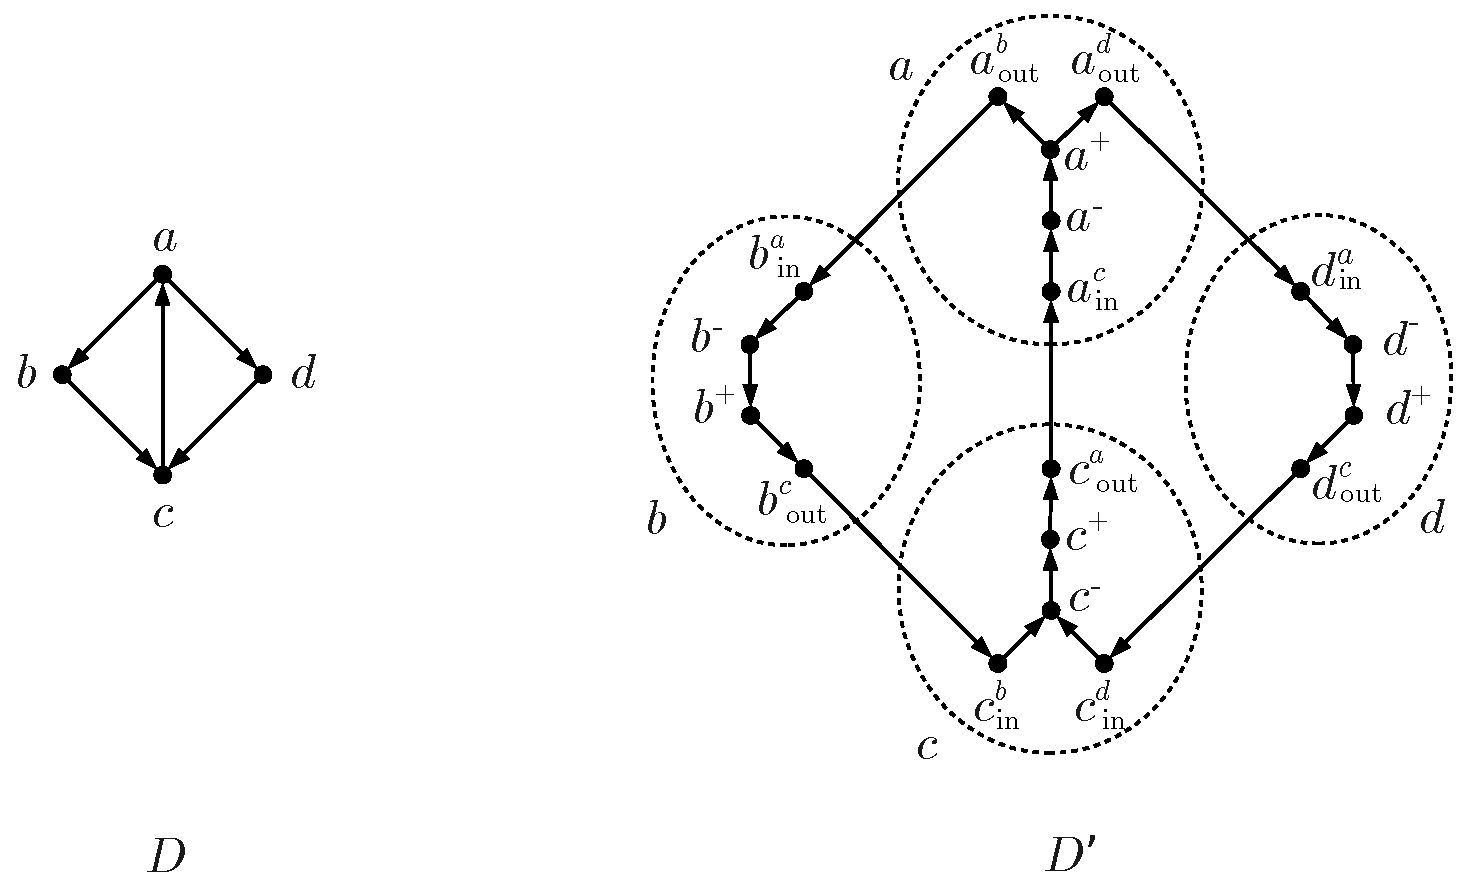
\includegraphics[scale=.45]{../figs/fig_reduction1}
    \caption{An instance~$D$ of DFVS and the modified graph~$D'$.}
    \label{fig:reduction1}
\end{figure}

We now first show that~$D$ has a FVS of size at most~$f$ if and only if~$D'$ has a FVS of size at most~$f$. Observe that each directed cycle of~$D$ corresponds to a directed cycle of~$D'$ and vice versa. Also notice that any cycle in $D'$ that contains a vertex $v_{\text{in}}^{u}$ or a vertex $v_{\text{out}}^{w}$ also contains the vertices $v^-$ and $v^+$. Hence, for any FVS~$F$ of~$D'$ we can create a FVS~$F'$ of $D'$ of at most the same size and containing only vertices of the type $v^-$. We assume from now on that any FVS of $D'$ is of this form. It is now obvious that $F= \{ v\in V \mid v^- \in F'\} $ is an FVS of $D$ if and only if $F'= \{ v^-\in V' \mid v \in F\} $ is an FVS of $D'$.

Intuitively, the idea of our reduction is as follows. We will construct two rooted binary trees~$T_1$ and~$T_2$ consisting of long chains. We build them in such a way that the graph~$D'$ is basically the inheritance graph of the chain forest for $T_1$ and $T_2$. This graph can be made acyclic by atomizing some of the chains. Thus, solving {\sc DFVS} on~$D'$ is basically equivalent to deciding which chains to atomize. We make all the chains that can be atomized of the same length. Hence, since each chain that is atomized adds the same number of components to the agreement forest, solving {\sc DFVS} on~$D'$ is essentially equivalent to finding a maximum acyclic agreement forest for $T_1$ and $T_2$.

Before we proceed, we need some more definitions. Recall that an {\it $n$-chain} of a tree is an $n$-tuple $(a_1,a_2,\ldots,a_n)$ of leaves such that the parent of $a_1$ is either the same as the parent of $a_2$ or the parent of $a_1$ is a child of the parent of $a_2$ and, for each $i\in\{2,3,\ldots,n-1\}$, the parent of $a_i$ is a child of the parent of $a_{i+1}$. A tree~$T$ whose leaf set~$\cL(T)$ is a chain of~$T$ is called a \emph{caterpillar} on~$\cL(T)$\footnote{{In this context a caterpillar does \emph{not} have an artificial vertex labelled $\rho$.}} It is easy to see that, for every chain~$C$, there exists a unique caterpillar on~$C$.  By \emph{hanging} a chain~$C$ below a leaf~$x$, we mean the following: subdivide the edge entering~$x$ by a new vertex~$v$ and add an edge from~$v$ to the root of the caterpillar on~$C$. When we hang a chain~$C_1$ below a chain~$C_2$, we hang the caterpillar on~$C_1$ below the lowest leaf (or a lowest leaf)~$x_1$ of~$C_2$. By \emph{replacing} a leaf~$x$ by a 
chain~$C$ we mean: delete~$x$ and add an edge from its former parent to the root of the caterpillar on~$C$.

We are now ready to construct an instance of {\sc MAAF}. The trees,~$T_1$ and~$T_2$, will be built of chains of three types: x-type, y-type and z-type. The x-type chains have length~$\ell$ while the y-type and z-type chains have length~$L$ (with $L>>\ell$). Each of these chains will be common to both trees. Recall that,
by Lemma~\ref{lem:survives}, we may assume that every chain either survives or is atomized. The idea is that y-type chains and z-type chains are so long that they will all survive. The x-type chains are shorter and might be atomized. In fact, the x-type chains that are atomized will correspond to a FVS of~$D'$.

\begin{figure}
    \centering
    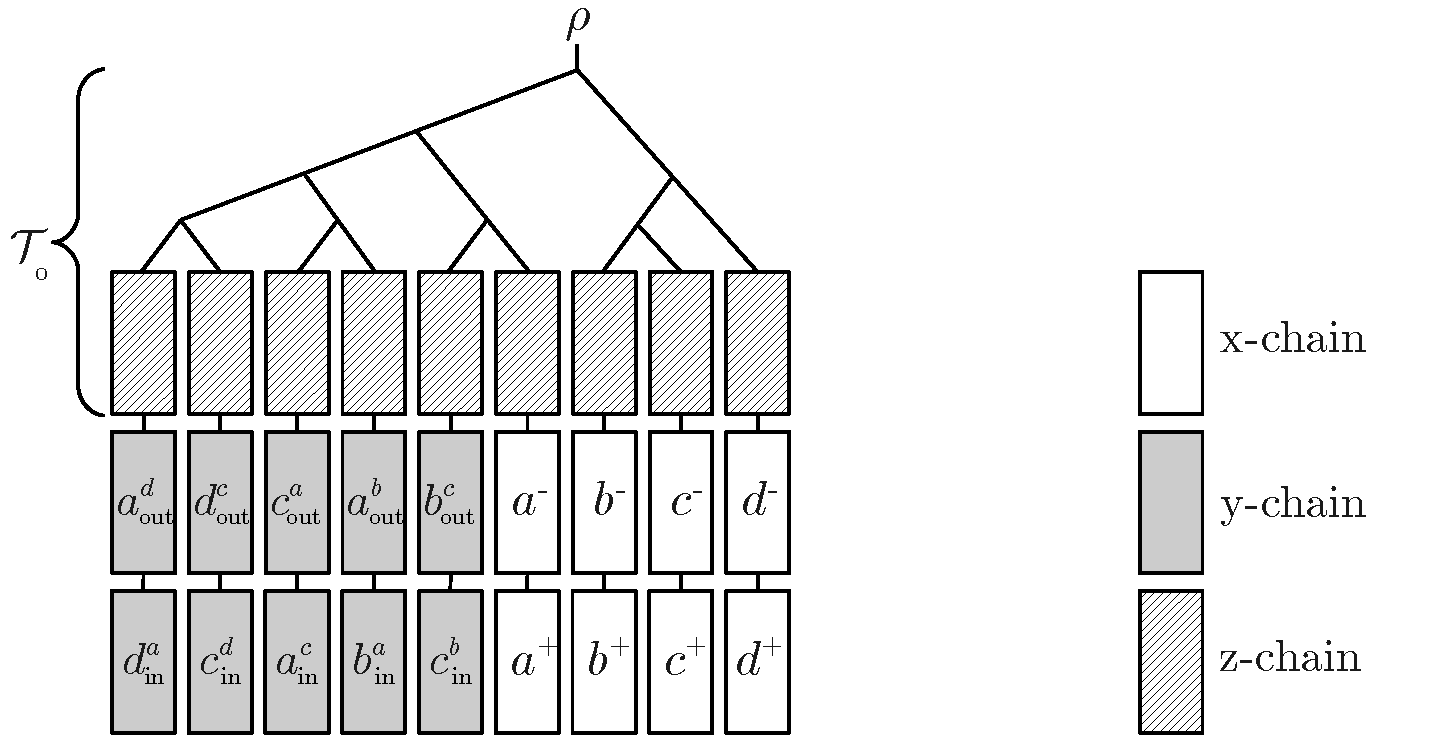
\includegraphics[scale=.5]{../figs/fig_reduction2}
    \caption{$T_1$: the first tree of the constructed MAAF instance.}
    \label{fig:reduction2}
\end{figure}

\begin{figure}
    \centering
    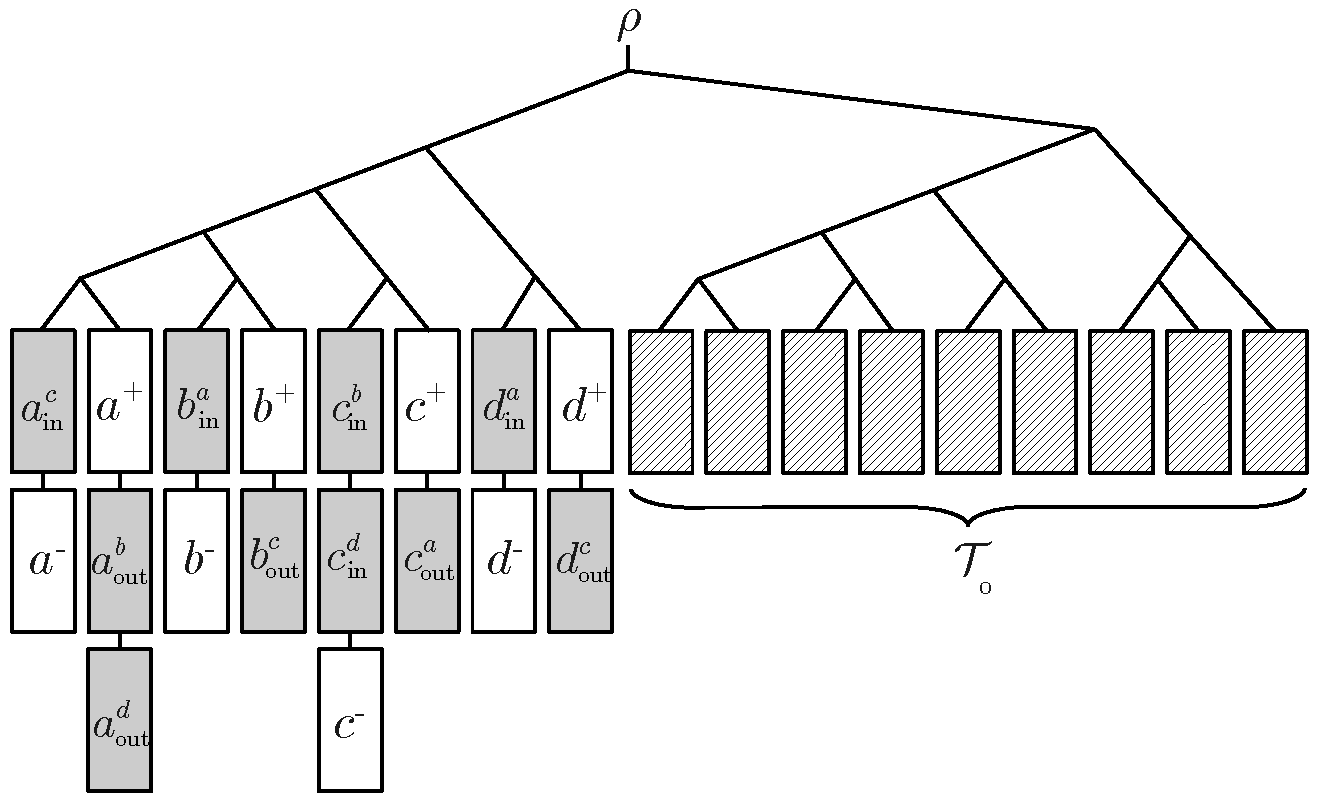
\includegraphics[scale=.5]{../figs/fig_reduction3}
    \caption{$T_2$: the second tree of the constructed MAAF instance.}
    \label{fig:reduction3}
\end{figure}

We build the trees~$T_1$ and~$T_2$ as follows. For each vertex of~$D'$ of the type~$v^-$ or~$v^+$ we create an x-type chain. For each other vertex of~$D'$ we create a y-type chain. Finally, for each vertex and edge of the original graph~$D$ we create a z-type chain. All leaves of all chains have different labels. Now we combine the chains into two trees as follows.

First~$T_1$. Start with an arbitrary rooted binary tree on~$|V|+|A|$ leaves labeled by the vertices and edges of $D$. We replace each leaf by its z-type chain, creating the tree which we call $T_0$. Below each z-chain replacing a leaf labeled by an edge $(u,v)\in A$ we hang the y-type chain for~$u_\text{out}^v$ and below that the y-type chain for~$v_\text{in}^u$. Below each z-chain replacing a leaf labeled by a vertex $v\in V$ we hang a x-type chain for~$v^-$ and below that a x-type chain for~$v^+$. 

Now~$T_2$. Start with an arbitrary rooted binary tree on~$2|V|$ leaves having two leaves for each vertex~$v\in V$. Replace one of them by a concatenation of (from top to bottom) the y-type chains for $v_{\text{in}}^{u_1},v_{\text{in}}^{u_2},\ldots,v_{\text{in}}^{u_{d^-(v)}}$ and the x-type chain for~$v^-$. Replace the other leaf for~$v$ by a concatenation of (from top to bottom) the x-type chain for~$v^+$ and the y-type chains for $v_{\text{out}}^{w_1},v_{\text{out}}^{w_2},\ldots,v_{\text{out}}^{w_{d^+(v)}}$. Finally, hang a copy of~$T_0$ below the root. This concludes the construction of the MAAF instance. For an example, see Figures~\ref{fig:reduction2} and~\ref{fig:reduction3}.

We claim that~$D'$ (and thus~$D$) has a FVS of size at most~$f$ if and only if there exists an acyclic agreement forest of~$T_1$ and~$T_2$ of size at most $1+2(|A|+|V|)+(\ell-1)f$.

To show this, consider the agreement forest~$A_D$ for~$T_1$ and~$T_2$ in which~$T_0$ is one component, each x-type chain is one component, and each y-type chain is one component. Represent the components of $A_D$ by their corresponding vertices and edges. The inheritance graph $G_{A_D}$ is obtained from $D'$ by adding the edges $(v_{\text{in}}^{u_i},v_{\text{in}}^{u_j})$ for all $1\leq i< j\leq d^-(v)$,  the edges $(v_{\text{out}}^{w_i},v_{\text{out}}^{w_j})$ for all $1\leq i< j\leq d^+(v)$, and creating a vertex $v_{T_0}$ corresponding to $T_0$ with only outgoing edges to all other vertices. Hence $v_{T_0}$ is not in any cycle of $G_{A_D}$.
It is easy to see that any FVS of $D'$, which by assumption has only vertices of the type $v^-$, is also a FVS of $G_{A_D}$ and vice versa, since any directed cycle of $G_{A_D}$ passing through an edge $(v_{\text{in}}^{u_i},v_{\text{in}}^{u_{i+1}})$ or $(v_{\text{out}}^{w_i},v_{\text{out}}^{w_{i+1}})$
must contain $v^-$. In addition, since $v^-$-type vertices correspond to x-type chains, it is possible to make~$G_{A_D}$ acyclic by atomizing only x-type chains.

Let~$F$ be a FVS of~$D$ and let~$F'$ be the corresponding FVS of~$D'$. Then we can construct an agreement forest~$\cR$ of~$T_1$ and~$T_2$ as follows. One component consists of the tree~$T_0$. Each of the y-type chains is also one component, as well as each x-type chain that does not correspond to a vertex in~$F' $. Finally, each x-type chain corresponding to a vertex in~$F'$ is atomized. Thus, the number of components is $1+2|A|+(2|V|-|F'|)+\ell|F'| = 1+2(|A|+|V|)+(\ell-1)|F|$. We have to show that the inheritance graph $G_\cR$ is acyclic. We can construct $G_\cR$ from~$G_{A_D}$ as follows. Delete every vertex~$v^-\in F'$ and instead add a vertex for each leaf of the corresponding x-type chain with incoming edges from~$T_0$ and from $v_{\text{in}}^{u_1},v_{\text{in}}^{u_2},\ldots,v_{\text{in}}^{u_{d^-(v)}}$. Since we only introduced leaves with incoming edges, this modification does not create any directed cycles. Thus, since~$F'$ contains a vertex of each directed cycle of~$G_{A_D}$, 
and all vertices from~$F'$ have been removed, $G_\cR$ is acyclic. It follows that~$\cR$ is an acyclic agreement forest for~$T_1$ and~$T_2$.

To show the other direction, let~$\cA$ be an acyclic agreement forest of~$T_1$ and~$T_2$. First, we may assume that all y-type chains and z-type chains survive in~$\cA$, since we will choose~$L$ sufficiently large (as will be specified later). To see this, recall that we may assume by Lemma~\ref{lem:survives} that each chain either survives or is atomized. Hence, if a y-type chain or z-type chain does not survive, it is atomized and adds~$L$ components to the agreement forest. Secondly,  observe that we may assume that all z-type chains are together in a single component (if they are not, we can put them together and reduce the number of components). 

Now we argue that any pair of chains, {at least} one of which is not a z-type chain, cannot be together in a single component of~$\cA$. Firstly, if the two chains are below each other in~$T_1$, then they are next to each other in~$T_2$. Secondly, if the two chains are next to each other in~$T_1$, then they are separated by a z-type chain in~$T_1$ but not in~$T_2$. Hence, by~(2) in the definition of an agreement forest, the two chains can not be together in a single component of~$\cA$. Thus, the components of~$\cA$ are as follows. Tree~$T_0$ is the component containing the root and all z-type chains. Furthermore, each y-type chain, each surviving x-type chain, and each leaf of a non-surviving x-type chain is a separate component. Let~$\tilde{F}$ be the set of vertices of~$G_{A_D}$ corresponding to the non-surviving x-type chains. Thus, each vertex in~$\tilde{F}$ is of the type~$v^-$ or~$v^+$. We will show that~$\tilde{F}$ is a FVS of~$G_{A_D}$ and hence of~$D'$. We can construct $G_{\cA}$ 
from $G_{A_D}$ as follows. Remove each vertex in~$\tilde{F}$ from~$G_{A_D}$ and add each leaf of the corresponding x-type chain as a separate vertex. Then add edges to these newly added vertices (these edges are not important since they do not create any directed cycles). Since~$\cA$ is an acyclic agreement forest, $G_\cA$ is acyclic and hence~$\tilde{F}$ is a FVS. The size~$|\tilde{F}|$ of the FVS is equal to the number of non-surviving x-type chains. Thus, $|\cA| = 1+2|A|+(2|V|-|\tilde{F}|)+\ell|\tilde{F}| = 1+2(|A|+|V|)+(\ell-1)|\tilde{F}|$.

The reduction is clearly polynomial time. It remains to show that it is approximation preserving. Suppose that there exists a $c$-approximation algorithm for {\sc MAAF}. Say that~$m$ is the size of the MAAF returned by this algorithm and~$m^*$ the size of an optimal solution. Recall that {\sc MAAF} minimizes the size of an agreement forest minus one, so $m-1\leq c\cdot (m^*-1)$. We have shown that~$D$ has a FVS of size at most~$f$ if and only if~$T_1$ and~$T_2$ have an acylic agreement forest of size at most $1+2(|A|+|V|)+(\ell-1)f$. Thus, $m^*=1+2(|A|+|V|)+(\ell-1)f^*$. Moreover, an approximate solution~$f$ of DFVS can be computed from an approximate solution~$m$ of MAAF by taking $f = ( m - 1 - 2(|A|+|V|) ) / (\ell-1)$. Then we have

\begin{eqnarray*}
f & = & \frac{m - 1 - 2(|A|+|V|)}{\ell-1}\\
& \leq & \frac{c\cdot (m^* - 1) - 2(|A|+|V|)}{\ell-1}\\
& = & \frac{c(2(|A|+|V|)+(\ell-1)f^*)-2(|A|+|V|)}{\ell-1}\\
& = & c\cdot f^* + \frac{2(c-1)(|A|+|V|)}{\ell-1}\\
& = & c\cdot f^* + 1\\
\end{eqnarray*}

if we take $\ell = \lceil2(c-1)(|A|+|V|)+1\rceil$. We still need to specify the value of~$L$, which needs to be sufficiently large so that all y-type chains and z-type chains survive. Since any graph trivially has a FVS of size~$|V|$, any constructed {\sc MAAF} instance has $m^*\leq 1+2(|A|+|V|)+(\ell-1)|V|$. Thus, a $c$-approximation algorithm will return an acyclic agreement forest of size~$m$ with $m-1\leq c(m^*-1) \leq c(2(|A|+|V|)+(\ell-1)|V|)$. And hence with~$m\leq c(2(|A|+|V|)+(\ell-1)|V|)+1$. So it suffices to take $L = \lceil c(2(|A|+|V|)+(\ell-1)|V|) + 2\rceil$.

Now take $\epsilon > 0$. If $f^*<1 / \epsilon$, we can compute an optimal solution for {\sc DFVS} by brute force in polynomial time. Otherwise, $1 \leq  \epsilon\cdot f^*$ and we have

\[
f \leq c\cdot f^* + \epsilon\cdot f^* = (c+\epsilon)f^*.
\]

Thus, if there exists a $c$-approximation for MAAF, then there exists a $(c+\epsilon)$-approximation for DFVS for every fixed~$\epsilon > 0$.

\end{proof}

In contrast to the result in Section~\ref{sec:2dfvs}, the reduction above can only be used for constant~$c$. It does \emph{not} show that e.g. an $\text{O}(\log |X|)$-approximation for \mh would imply an $\text{O}(\log |V|)$-approximation for {\sc DFVS}. Hence, it is indeed possible that \mh admits an $\text{O}(\log |X|)$-approximation while {\sc DFVS} does not admit an $\text{O}(\log |V|)$-approximation. For neither of the problems such an approximation is known to exist.

Finally, we note that Theorem \ref{theorem:dfvsToHybrid} also allows
us to improve upon the best-known inapproximability result for \mh.

\begin{corollary}
There does not exist a polynomial-time $c$-approximation for \mh, where
$c < 10\sqrt{5}-21 \approx 1.3606$, unless P=NP. If the Unique Games Conjecture
holds, then there does not exist a polynomial-time $c$-approximation for \mh where
$c < 2$.
\end{corollary}
\begin{proof}
In \cite{karp1972} a simple reduction is shown from the problem \textsc{Vertex Cover}
to the problem {\sc DFVS}. Specifically, given an undirected graph $G$ as input to \textsc{Vertex Cover} we create a directed graph $G'$ by transforming each edge $\{u,v\}$ in $G$ into two directed edges
$(u,v), (v,u)$ in $G'$. It is easy to show that $G'$ has a feedback vertex set of size
$k$ if and only if $G$ has a vertex cover of size $k$. Consequently, any polynomial-time
$c$-approximation algorithm for DFVS can be used to construct a polynomial-time
$c$-approximation for \textsc{Vertex Cover}. The latter problem does not permit a polynomial-time $c$-approximation, for any $c < 10\sqrt{5}-21 \approx 1.3606$, unless P=NP \cite{dinur,DinurAnnals}.
Also, it has been shown that if the Unique Games Conjecture is true then no approximation better than 2 is possible \cite{Khot2008}. Now, the proof of Theorem \ref{theorem:dfvsToHybrid} shows that, if there exists a $c$-approximation for \mh, then there exists a $(c+\epsilon)$-approximation for DFVS for \emph{every} fixed~$\epsilon > 0$. Hence the existence of a $c$-approximation for \mh where $c < 10\sqrt{5}-21$ (respectively, $c < 2$) would mean the existence of a $c'$-approximation for DFVS (and thus also for \textsc{Vertex Cover}) where $c' <  10\sqrt{5}-21$ (respectively, $c' < 2$).
\end{proof}




%\section{Conclusion}
We have seen several interesting spin-off consequences of the result presented in this chapter, both negative and positive. On the negative side, it is known that there is a very simple parsimonious reduction from the classical problem {\sc Vertex Cover} to DFVS \cite{karp1972}. Consequently, a $c$-approximation for DFVS entails a $c$-approximation for {\sc Vertex Cover}, for every $c \geq 1$. For $c < 10\sqrt{5}-21 \approx 1.3606$ there cannot exist a polynomial-time $c$-approximation of {\sc Vertex Cover}, assuming P $\neq$ NP \cite{dinur,DinurAnnals}. Also, if the Unique Games Conjecture is true then for $c < 2$ there cannot exist a polynomial-time $c$-approximation of {\sc Vertex Cover} \cite{Khot2008}. (Whether {\sc Vertex Cover} permits a constant factor approximation ratio strictly smaller than 2 is a long-standing open problem). The main result in this chapter hence not only showed that \mh is in APX if and only if DFVS is in APX, but also that \mh cannot be approximated within a factor of 1.3606, unless P=NP (and not within a factor smaller than 2 if the Unique Games Conjecture is true). This improves significantly on the current APX-hardness threshold of $\frac{2113}{2112}$.

On the positive side, we observe that already-existing approximation algorithms for {\sc DFVS} can be utilized to give asymptotically comparable approximation ratios for \mh. To date the best polynomial-time approximation algorithms for {\sc DFVS} achieve an approximation ratio of $\text{O}( \min\{ \log n \log \log n, \log \tau^{*} \log \log \tau^{*}\} )$, where $n$ is the number of vertices in the graph and $\tau^{*}$ is the optimal fractional solution of the problem (taking the weights of the vertices into account) \cite{dfvsApprox,dfvsSeymour}. We showed that this algorithm can be used to give an $\text{O}( \log r \log \log r )$-approximation algorithm for \mh, where $r$ is the hybridization number of the two input trees. To the best of our knowledge, this is the first non-trivial polynomial-time approximation algorithm for \mh.


On the practical side, we realized that our insight into cycle breaking leads to a cute, simple and increadibly good approximation algorithm. In the next two chapters we improve on the theoretical work done here, present two algorithms and run experiments to convince the reader of just how good this algorithm is in practice. 

% The main result also had interesting consequences for the fixed parameter tractability of \mh. We saw that the inflation factor of 6 in the reduction from {\sc DFVS} to \mh was very closely linked to a reduction described by Bordewich and Semple~\cite{bordewich07b}. They showed that the input trees can be reduced to produce a weighted instance containing at most $14r$ taxa which we have sharpened to at most $9r$ taxa. Without this sharpening, the inflation factor we obtain would have been higher than 6. From this analysis it becomes clear that the kernel size has an important role to play in analysing the approximability of \mh.
% 
% This raises some interesting general questions about the linkages between \mh and {\sc DFVS}. For example, the reduction by Bordewich and Semple, which gives a linear kernel for a weighted variant of \mh, can be modified slightly (as is e.g. done in~\cite{bonet10} for unrooted SPR distance) to obtain a quadratic kernel for \mh (without weights). This contrasts sharply with {\sc DFVS}. It is known that {\sc DFVS} is fixed parameter tractable~\cite{dfvsFPT}, but it is \emph{not} known whether {\sc DFVS} permits a polynomial-size kernel. Might \mh give us new insights into the structure of {\sc DFVS} (and vice-versa)? More generally: within which complexity frameworks is one of the two problems strictly harder than the other?
